
\chapter{Introduction}
\label{cha:introduction}

This chapter presents the general context of the project, the problem found and offers a brief explanation of the proposed solution. It ends with a description of the document structure.

\section{Context}
\label{s:context}

Traditionally, people looking for a new place to live would focus on the characteristics of the estate. Nowadays people attribute equal importance to everything surrounding the place they intend to live in~\cite{Montezuma2019}, with the needs and limitations of each family dictating their choices. This resource limitations, whether time or money, have to be incorporated into the ordering in which the houses are presented. While also accounting for their social needs, however, as of now, most real estate websites do not reflect this reality and are not presenting this type of data to the user.

Current real estate websites also struggle with the dynamism of the data, where houses are constantly being added and removed from the market, resulting in constant pricing updates making it difficult to the user to keep track. \\

Lastly, each real estate website contains different information regarding the houses they display. This introduces a new challenge, as the integration process becomes more complex since it needs to be abstract enough to contemplate all real estate websites information and specific enough to extract the necessary information to filter estates according to the needs of each family, social or estate related.

Therefore the goal is to find a way to tackle this problem, using development strategies that could make the system modular and scalable.

\section{Objetives}
\label{s:objectives}
% \begin{itemize}
%     \item desenvolver uma plataforma de pesquisa de casa
%     \item classificar casas de acordo com as necessidade dos users
%     \item desenvolver um sistema de extração de dados
%     \item agregar e integrar dados de multiplas plataformas
%     \item desenvolver um sistema escalavel e modular
%     \item garantir o bom funcionamente da plataforma atravez de testing e monitorização
    
%     \item providenciar uma experiencia interativa e intuiva ao user na procura de casa atraves da UI
    
% \end{itemize}

The ultimate goal of this thesis was to develop a platform to search for real estate considering the needs of its users, measured by a life quality index. This needs can be split into two categories, social or estate related. Which means its not only concerned with the estate itself but also the needs of each family, for instance, a user may prefer to live close an hospital while another may prefer to live near an entertainment center. And to understand the needs of each family, we developed Index, a life quality index that rates each estate according to the users preferences, which means each estate has a different rating for each user. \\

To accomplish this we acquired information from real estate and \acrfull{poi} surrounding this estates. The real estate data was not publicly available and as such, to obtain it, a scrapper was created with the goal of periodically collecting data from multiple real estate websites. While the \acrshort{poi} data was gathered from Lisbons' open data platform, \textbf{Lisboa Aberta} \footnote{\url{http://lisboaaberta.cm-lisboa.pt/index.php/pt/}}. 

Since most websites store their information in a distinct manner, all the estate information gathered had to be aggregated and integrated into the system following an unique data model created for our platform, ready to accommodate current and future changes. \\

The second goal was to create a modular system, that through modern technologies and strategies, would help ups guarantee a system implementation that could easily be scalable while maintaining high availability. To ensure this, a monitoring system was put in place that helps reduce downtime by allowing for faster error discovery and recovery, by having the overall health of system all in one place. \\

Lastly, it was important that the platform would provide an interactive and intuitive user experience to the user looking for a new estate, therefore the user interface was designed to be pleasant and fun to use with a lot of visual elements, and more importantly, easy to use and to understand


\section{Solution}
\label{s:proposed_solution}

We based our solution on the concept of the 15 minutes city. According to Carlos Moreno a 15-minute city is a residential urban concept in which most daily necessities can be accomplished by either walking or cycling from residents homes~\cite{15mincity}. This idea rides on the concept of "chrono-urbanism", which outlines that the quality of urban life is inversely proportional to the amount of time invested in transportation, more so through the use of automobiles. Moreno advocates for locations where locals can access all their basic needs at distances that would not take them more than 15 minutes by foot or by bicycle. For this concept, Moreno supports that citizens will be able to enjoy a higher quality of life where they will be able to effectively fulfil six essential urban social functions to sustain a decent urban life~\cite{smartcities4010006}. Those include:

\begin{itemize}
    \item Living
    \item Working
    \item Commerce
    \item Healthcare
    \item Education
    \item Entertainment
\end{itemize}

This idea was incorporated on this thesis by classifying all estates in the platform according to the users needs. This method considers the distance from each house to the surrounding \acrshort{poi}s and classifies the estate according to the users preferences. For instance, if a certain estate is close to a hospital it will have a low classification score for a user that has healthcare on the bottom of its priorities. On the other hand the house will have a high score for a user that has healthcare as its top priority. This system provides a more complete search as it considers the life quality that the users are trying to achieve. 

The classification system is a way of quantifying life quality, translated to a score that we call Index. It requires users to explicitly define their preferences regarding their ideal home surroundings. Therefore, Index is a number (0 to 100) that describes 
if an estate fits a person or not, according their personal preferences, being 100 the best possible score. \\

To produce Index, estate information was gathered from several real estate websites and the \acrshort{poi}s data was gathered from Lisbons' open data platform, \textbf{Lisboa Aberta} \footnote{\url{http://lisboaaberta.cm-lisboa.pt/index.php/pt/}}. \\

We developed a platform that allows users to search estates and their corresponding Index results. The platform was made to have a slick and intuitive design where the users could easily find what they were looking for. To process all this we implemented a microservices architecture. This pattern is modular by nature and facilitates updates, since only the new feature needs to be deployed. It is a better approach when compared to a monolithic architecture, since the latter requires the entire project to be redeployed, instead of deploying only the necessary component. This is a symptom that gets worse, the bigger the application gets. The monolithic approach also makes scaling difficult, as the entire application must be scaled instead of only scaling the necessary components~\cite{7333476}. This means that typical monolithic applications does not keep up now with the current demand of users~\cite{7458761}. 

The microservice pattern facilitates this problem by defining each of the smaller components as their own service called microservices --- independent processes that implement a certain functionality and that can communicate with other microservices to provide more complex functionality.

This pattern solves some of the previously mentioned problems. Deploying new features becomes easier, as it is now possible to deploy only the new feature without having to redeploy the entire application. It is possible to ensure that this deployments do not break the application by having predefined tests in place that guarantee the systems integrity. As each service is independent, it can also be deployed multiple times with multiple resource configurations, making the system scalable with ease. 

Finally, we used a monitoring system to help us deal with possible flaws or failures.

\begin{comment}


---------------------------------------------------------------------------






% In the technical point of view, typical development of applications does not keep up now with the current demand of users~\cite{7458761}. In a typical monolithic architecture, it is not possible to deploy the application efficiently, as to deploy the application the entire application must be redeployed, instead of deploying only the modified component, a symptom that gets worse, the bigger the application gets. This approach makes scaling difficult, as the entire application must be scaled instead of only scaling the necessary components~\cite{7333476}. \\



%\todo[inline]{extender. o texto que tirei do artigo}

%Even though that in most of the definitions available, the concept don't consider cars as a travel option, since it extends the range by several kilometers, we have decided to give the user that decision while presenting the disadvantages of such choices.

% Requirements Objetivo era ser completamente escalavel
%Since our priority was to make the architecture scalable (product and team wise)  with high availability, one of the first decisions made towards this goal was to have an underlying architecture based on microservices, which would allow independently scalable and deployable services. Having everything isolated, also contributes to reduce downtime through fault isolation. 
%To deploy this solution, we set as a requirement that each of our services should be containerized with Docker and deployed in Kubernetes. With kubernetes, we had at our disposal tools that allowed each service to be deployed as pod that could automatically be scaled up and down in a matter of seconds, which allows us to target specific microservices that may require an extra performance boost. 
%As the application requires real estate information and points of interest (POI) surrounding such estates, we had to come up with a solution to gather all this information. So, we designed a scraping solution to collect data from multiple real estate websites. For relevant POI, most of the information was publicly available, so we gathered the data needed from Lisbon's open data platform, \textbf{Lisboa Aberta} \footnote{\url{http://lisboaaberta.cm-lisboa.pt/index.php/pt/}}.

% Explicar que para isso são precisos dados, e nao foi facil de obter
%The main goal of the application is to present users with multiple estates and help them decide the best fit, and as such data has a big role. Too ensure we had enough information, we had to gather estate data and relevant information to the areas that surround such estates. Since there was no publicly available information, a web scraping solution was designed to periodically collect data from multiple real estate websites, such as \textbf{Remax} \footnote{\url{https://www.remax.pt/}} and \textbf{Imovirtual} \footnote{\url{https://www.imovirtual.com/}}. For relevant points of interest (POI) in the surrounded environment, and as a proof of concept, we gathered data mostly from Lisbon, provided by \textbf{Lisboa Aberta} \footnote{\url{http://lisboaaberta.cm-lisboa.pt/index.php/pt/}}, an open data platform for the city of Lisbon.
In Figure~\ref{fig:arc-overview}, we can see an overview of our project architecture and its most important components.

\begin{figure}[t]
	\centering
	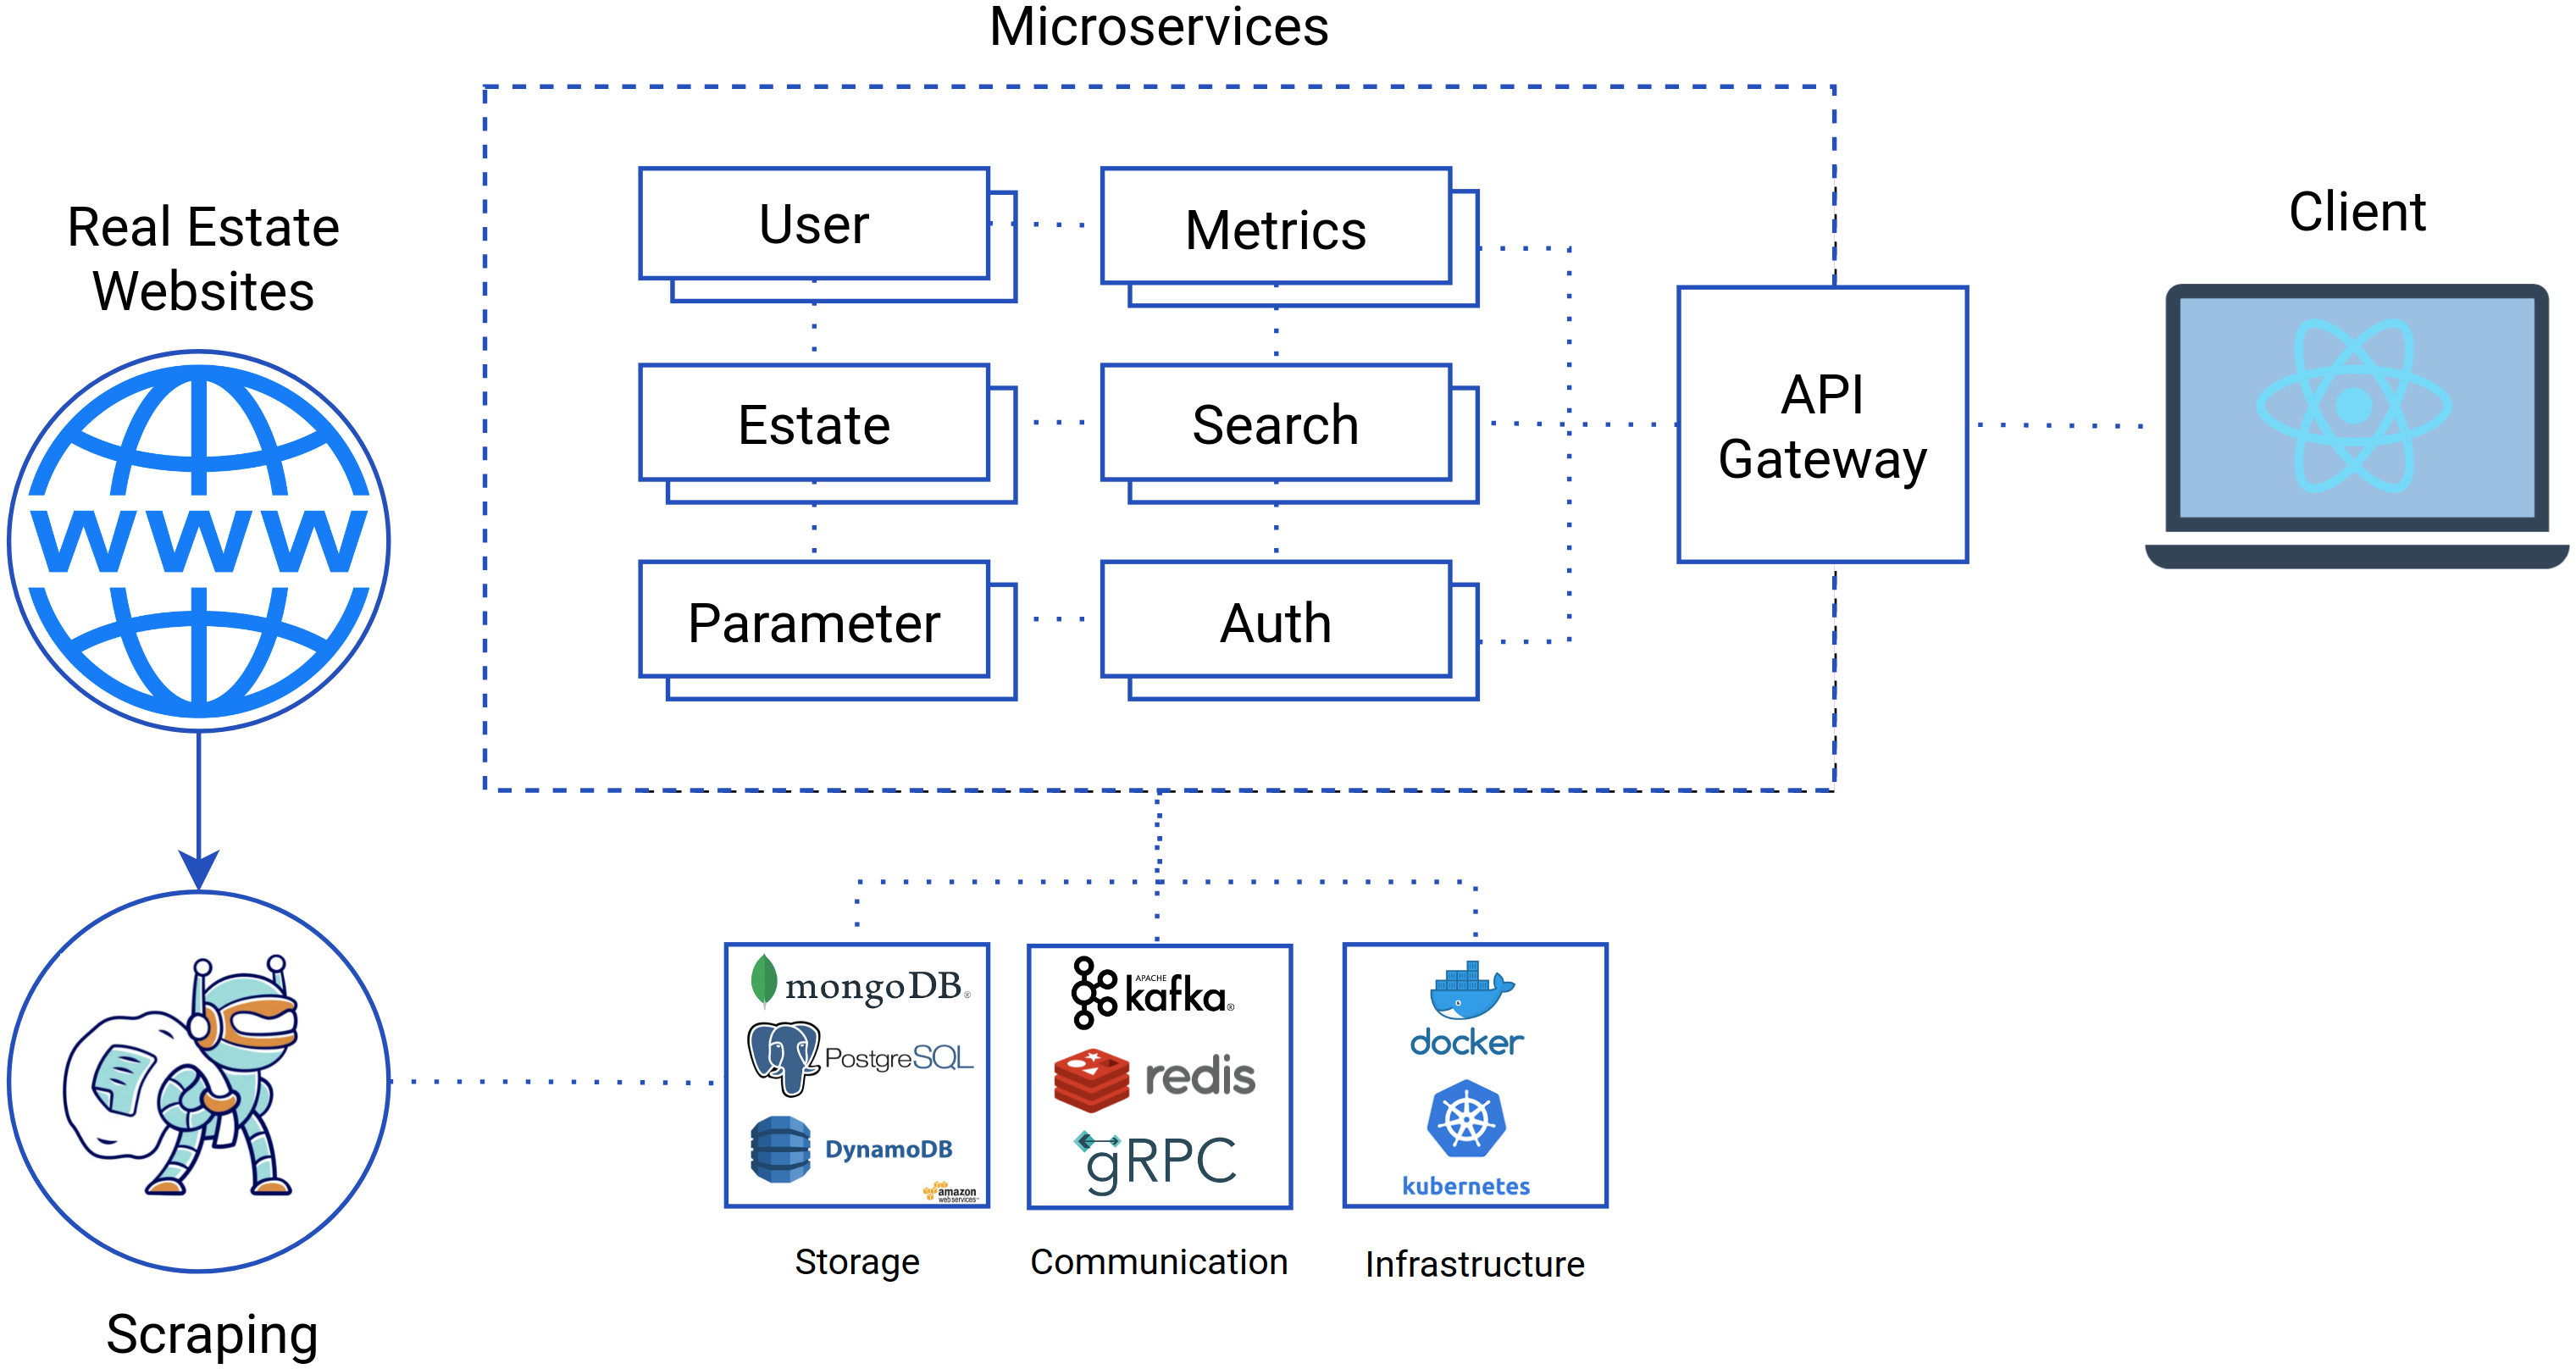
\includegraphics[width=1\textwidth,clip,trim=0 0 0 0]{Chapters/img/introduction/arch_overview.png}
    \caption{Project architecture} 
    \label{fig:arc-overview}
\end{figure}

The first component is the data source, representing the real estate websites that are in turn scraped by our solution and inserted into the databases of one of our services. The microservices section is composed by all the required services, namely:

\begin{itemize}
    \item \emph{User}, used to access the users' personal information,
    \item \emph{Metrics}, responsible for the index logic and estate metrics,
    \item \emph{Estate}, access to all the property data,
    \item \emph{Search} allows us to perform text queries and easily find locations by name,
    \item \emph{Parameter} gives us access to the POI information, and
    \item \emph{Auth}, provides authentication and authorization, enabling user access to the website and to our services.
\end{itemize}

All services have their own databases, designed to support service specific use cases, and different ways of communicating. All services are funneled in through the API gateway, which receives requests from a React client.

\todo{tirei isto do contexto}Our system is a software solution developed to address the lack of information surrounding the process of buying a new estate, as described above. This system relies on data gathered from real estate websites, such as prices and locations. However, this data is constantly changing, as estates are constantly being added, removed and updated, as such our platform reflects this updates as well.

%=======================================================================
\end{comment}


\section{Structure}
\label{s:thesis_outline}

The rest of the document is organized in the following chapters:

\begin{itemize}
    \item \textbf{Background and Related Work} --- Description of the current implementations in the scientific world, followed by some of the key concepts and finally some real life examples of similar systems;
    \item \textbf{15 Minute City} --- This chapter describes the technologies currently available to address each component, and a detailed account of how each of the problems was solved. 
    \item \textbf{Testing} --- Definition of the evaluation metrics intended to evaluate the scalability of the system and a detailed description of the performed tests;
    \item \textbf{Conclusion} --- Summary of the implementation and presentation of possible future work.
\end{itemize}
